\href{http://peeragogy.org/wp-content/uploads/2012/04/Bryan.jpg}{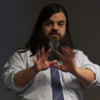
\includegraphics{http://peeragogy.org/wp-content/uploads/2012/04/Bryan.jpg}} \textbf{Bryan
Alexander -- USA, VT} \textbf{Author} I research the ways new
technologies change education, teaching, learning, and scholarship. I'm
passionate about storytelling, gaming, pedagogy, and understanding the
future. My family homesteads on top of a little mountain, raising food.

Reach~\href{https://twitter.com/\#!/BryanAlexander}{Bryan on Twitter}
\textbar{} \href{http://bryanalexander.org/}{Bryan's personal website}

~ \textbf{Paul Allison -- USA,
NY} \textbf{\href{http://peeragogy.org/wp-content/uploads/2012/04/Paul.jpg}{
\includegraphics{http://peeragogy.org/wp-content/uploads/2012/04/Paul.jpg}}
Author} I teach at the~\href{http://bronxbash.com}{Bronx Academy Senior
High}, I'm part of the~\href{http://nycwritingproject.org}{New York City
Writing Project}, and I'm the NYC Technology Liaison for
the~\href{http://nwp.org}{National Writing Project}. I help
manage~\href{http://youthvoices.net/}{Youth Voices} and I co-produce
\href{http://teachersteachingteachers.org}{Teachers Teaching Teachers}.

Reach~\href{https://plus.google.com/u/0/113993022447291199374/about}{Paul
on Google+} \textbar{} \href{http://teachersteachingteachers.org}{Paul's
personal website}

~ \textbf{María F. Arenas -- República
Argentina} \textbf{\href{http://peeragogy.org/wp-content/uploads/2012/04/Maria.jpg}{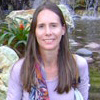
\includegraphics{http://peeragogy.org/wp-content/uploads/2012/04/Maria.jpg}}}
\textbf{Author, Editor} Independent consultant researcher on TICS
applied to Learning, Digital Communication, Institutional, Corporate. On
line facilitator tutorship. Professor on Semiotics, Social
Communication, Networking. Non Violent Communication.

Reach~\href{https://plus.google.com/u/0/stream/circles/p2e54657d0d6fc86d}{María~on
Google+} ~\textbar{}
\textbf{~}\href{http://arenastudies.wordpress.com/}{María's personal
website}

~
\textbf{\href{http://peeragogy.org/wp-content/uploads/2012/04/Regis.jpg}{
\includegraphics{http://peeragogy.org/wp-content/uploads/2012/04/Regis.jpg}}Régis
Barondeau --~Canada}\textbf{Author} I build bridges between research,
praxeology and technology and I become creative ``by finding a likeness
between things which were not thought alike before'' (Bronowski, 1958).
I'm interested in complexity, culture, social media especially wikis,
education, open government and more.

Reach~\href{https://twitter.com/regisbarondeau}{Régis on Twitter}
\textbar{} \href{http://www.regisbarondeau.com}{Regis' personal website}

~
\textbf{\href{http://peeragogy.org/wp-content/uploads/2012/04/Doug.jpg}{
\includegraphics{http://peeragogy.org/wp-content/uploads/2012/04/Doug.jpg}}Doug
Breitbart -- USA, NJ Author, Meeting Support} I am first and foremost a
catalyst and provocateur who has worn the hats of attorney, consultant,
facilitator, coach, entrepreneur, father, husband, student, teacher, and
passionate believer in a networked, wired and semantic world.

Reach
\href{http://www.linkedin.com/profile/view?id=791427\&trk=tab_pro}{Doug
on LinkedIn} \textbar{} \href{www.ontologique.com}{Doug's personal
website}

~
\href{http://peeragogy.org/resources/meet-the-team/george/}{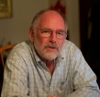
\includegraphics{http://peeragogy.org/wp-content/uploads/2012/04/George.jpg}}\textbf{George
Brett -- USA, VA Author, Editor, Meeting Support}

``Autodidactic techno arsty craftsy eclecticist.'' Many years as a
diplomat for IT technology as applied to research and education. I'm a
teacher/trainer, consultant, analyst, info ferret, artist, life-long
learner, and member of a great family. Looking for the best way to share
skills and experiences with others; and a Gen-Boomer seeking more steady
work.

Reach \href{http://www.linkedin.com/in/ghbrett/}{George on LinkedIn}
~\textbar{} ~\href{http://ghbrett.org}{George's personal website (NB:
archival)}

~
\textbf{\href{http://peeragogy.org/wp-content/uploads/2012/04/Suz.jpg}{
\includegraphics{http://peeragogy.org/wp-content/uploads/2012/04/Suz.jpg}}Suz
Burroughs -~USA, CA}\textbf{Author, Designer} I enable the connections
between the teacher and learner in all of us.
\href{http://www.learningsolutionsmag.com/articles/795/behavior-centered-design-at-google-a-case-study}{Learning
Designer},
\href{http://googleblog.blogspot.com/2012/12/unleashing-creativity-in-googles-csilab.html}{Design
Thinking facilitator},
\href{http://www.stmarytx.edu/news/top-stories/index.php?headline=Design_Thinking_Now_a_Part_of_MBA_Program}{Visiting
Professor of Innovation}, and \emph{Communitarian}.

Reach Suz on \ldots{} \textbar{}
~\href{http://susanburroughs.squarespace.com/}{Suz' personal website}

~
\textbf{\href{http://peeragogy.org/wp-content/uploads/2012/04/Joe.jpg}{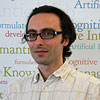
\includegraphics{http://peeragogy.org/wp-content/uploads/2012/04/Joe.jpg}}Joe
Corneli -- U.K.} \textbf{Author, Editor} Joseph Corneli is a Ph. D.
student at the Knowledge Media Institute of The Open University, UK,
where he does research on how people learn mathematics. He is a member
of the board of directors of the US-based nonprofit,
\href{planetmath.org}{PlanetMath.org}.

Reach~\href{http://identi.ca/arided}{Joe on Identi.ca} \textbar{}
\href{http://metameso.org/~joe\%20}{Joe's personal website}

~
\href{http://peeragogy.org/resources/meet-the-team/jay/}{
\includegraphics{http://peeragogy.org/wp-content/uploads/2012/04/Jay.jpg}}

\textbf{Jay Cross -- USA, CA} \textbf{Author}

Jay is the Johnny Appleseed of informal learning.
The~\href{http://internettimealliance.com/}{Internet Time Alliance},
which he chairs, helps corporations and governments use networks to
accelerate performance.

Reach \href{mailto:jaycross@internettime.com}{Jay by email}~\textbar{}
\href{http://jaycross.com}{Jay's personal website}

~
\textbf{\href{http://peeragogy.org/wp-content/uploads/2012/04/Charlie.jpg}{
\includegraphics{http://peeragogy.org/wp-content/uploads/2012/04/Charlie.jpg}}Charles
Jeffrey Danoff --~USA, IL} \textbf{Author} Charles is the Owner of Mr.
Danoff's Teaching Laboratory, an Educational Publishing and Services
firm he established in 2009. With Joe Corneli, he started publishing
research on Paragogy, Peeragogy's inspiration, in late 2010.

Reach~\href{http://identi.ca/mrd}{Charles on Identi.ca} ~\textbar{}
~\href{http://mr.danoff.org}{Charles' personal website}

~
\textbf{\href{http://peeragogy.org/wp-content/uploads/2012/04/James.jpg}{
\includegraphics{http://peeragogy.org/wp-content/uploads/2012/04/James.jpg}}James
Folkestad - USA, CO Author, Editor, Designer, Developer} My approach to
education has shifted from an emphasis on my teaching, to a more central
focus on student learning, and finally to an activity-systems approach
as I have come to realize that the two (teacher and learner) are
inseparable parts of the learning ecosystem.

Reach~\href{https://plus.google.com/u/0/114552232610071440407/about}{James
on Google+} ~\textbar{} ~\href{http://edgility.net}{James' personal
website}

~
\textbf{\href{http://peeragogy.org/wp-content/uploads/2013/10/John.jpg}{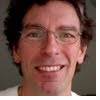
\includegraphics{http://peeragogy.org/wp-content/uploads/2013/10/John.jpg}}John
Graves, PhD - New Zealand Editor} Founder of
\href{http://slidespeech.com}{SlideSpeech}. Graduate of
\href{http://singularityu.org}{Singularity University}~and
\href{http://www.aut.ac.nz/}{AUT}.

Reach John on \href{http://twitter.com/slidespeech}{Twitter} \textbar{}
\href{http://slidespeech.tumblr.com}{Personal website}

~
\textbf{\href{http://peeragogy.org/wp-content/uploads/2012/04/Gigi.jpg}{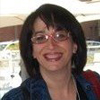
\includegraphics{http://peeragogy.org/wp-content/uploads/2012/04/Gigi.jpg}}Gigi
Johnson, EdD -- USA, CA Author, Developer} I mix formal learning
programs with programs to help learners begin to work, live, and create
everywhere. My own adventures include writing, singing, video, teaching,
and parenting 3 teens.

Reach~\href{http://twitter.com/maremel}{Gigi on Twitter} ~\textbar{}
~\href{http://maremel.com}{Gigi's personal page}

~
\textbf{\href{http://peeragogy.org/wp-content/uploads/2012/04/Anna.jpg}{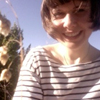
\includegraphics{http://peeragogy.org/wp-content/uploads/2012/04/Anna.jpg}}Anna
Keune -- Germany/Finland}\textbf{Co-author, Designer} I design
technology for learning and I like it.

Reach~\href{https://twitter.com/\#!/akeune}{Anna on Twitter} ~\textbar{}
~\href{www.annakeune.com}{Anna's personal website}

~
\href{http://peeragogy.org/resources/meet-the-team/kyle/}{\includegraphics{http://peeragogy.org/wp-content/uploads/2012/04/kyle.jpg}}\textbf{Kyle
Larson - USA, FL} \textbf{Editor} Kyle Larson is an undergraduate thesis
student at New College of Florida. His research interests include
composition theory, rhetorical theory, computers and composition, and
pedagogy.

Reach \href{https://plus.google.com/110988036495982155492/posts}{Kyle on
Google+}

~
\textbf{\href{http://peeragogy.org/wp-content/uploads/2012/04/Roland.jpg}{
\includegraphics{http://peeragogy.org/wp-content/uploads/2012/04/Roland.jpg}}Roland
Legrand -- Belgium Author} I'm a financial journalist, heavily involved
in experimenting with social media and new forms for reporting and
community conversation.

Reach~\href{http://www.twitter.com/rolandlegrand}{Roland on Twitter}
~\textbar{} ~\href{http://www.mixedrealities.com}{Roland's personal
website}

~
\textbf{\href{http://peeragogy.org/wp-content/uploads/2012/04/Amanda.jpg}{
\includegraphics{http://peeragogy.org/wp-content/uploads/2012/04/Amanda.jpg}}Amanda
Lyons --~\textbf{USA}, NY}\textbf{Designer} I am a Visual Practitioner,
Organization Development Consultant \& Experiential Educator. I love
helping people communicate via visual tools that generally include
markers and paper. I think our education system (in the U.S.) could
benefit from using visual communication tools as well as text based
methods to teach.

Reach~\href{https://twitter.com/\#!/amanda_lyons}{Amanda on Twitter}
~\textbar{} ~\href{www.visualsforchange.com/blog\%20\%20}{Amanda's
personal website}

~
\textbf{\href{http://peeragogy.org/wp-content/uploads/2012/04/Christopher.jpg}{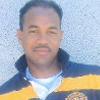
\includegraphics{http://peeragogy.org/wp-content/uploads/2012/04/Christopher.jpg}}Christopher
Neal -- USA, WA} \textbf{Communications and Media} I am driven by
technology and its ability to modify virtual communities and social
media. Coupled with a passion for Social:Learn, Social:iA, Situated
Cognition, Social Learning Theory, Connectivism and Collective
Intelligence etc.

Reach~\href{https://plus.google.com/u/0/106960445015668581969/posts}{Christopher
on Google+} \textbar{}
~\href{http://beyondcredentials.com/index.php?option=com_bc_profile_pages\&uname=berkeleyalum}{Christopher's
personal website}

~
\textbf{\href{http://peeragogy.org/wp-content/uploads/2012/04/Ted.jpg}{
\includegraphics{http://peeragogy.org/wp-content/uploads/2012/04/Ted.jpg}}Ted
Newcomb --~USA, AZ}\textbf{Author, Analytical project overview} Happily
retired grandpa, curating on digital culture, sociology of the web;
interested in collaboration and cooperation in digital networks that
result in positive change.

Reach \href{http://about.me/tcnewcomb}{Ted on About.me} ~\textbar{}
~\href{http://www.tcnewcomb.com}{Ted's personal website}

~
\textbf{\includegraphics{http://peeragogy.org/wp-content/uploads/2012/12/CP-Headshot.jpg}Charlotte
Pierce -- USA, MA}\textbf{Editor, Publisher} Indie publisher~who finds
in happiness in pushing her limits and seeing them back down. Augmented
her intellect in RheingoldU's
\href{http://socialmediaclassroom.com/host/think/}{Think-Know
Tools}~course, then joined the amazing Peeragogy community, where the
plot thickens.

Reach~\href{https://twitter.com/\#!/piercepress}{Charlotte on Twitter}
~\textbar{} ~\href{http://www.PiercePress.com}{Charlotte's personal
website}

~
\textbf{\href{http://peeragogy.org/wp-content/uploads/2012/04/Howard.jpg}{
\includegraphics{http://peeragogy.org/wp-content/uploads/2012/04/Howard.jpg}}Howard
Rheingold -- USA, CA}\textbf{Author, Editor} Inspired by Charles Danoff
and Joe Corneli's work on paragogy, I instigated the Peeragogy project
in order to provide a resource for self-organizing self-learners.
Learning is my passion.

Reach \href{https://twitter.com/\#!/hrheingold}{Howard on Twitter}
~\textbar{} ~\href{http://www.rheingold.com}{Howard's personal website}

~
\textbf{\href{http://peeragogy.org/wp-content/uploads/2012/04/Paola.jpg}{
\includegraphics{http://peeragogy.org/wp-content/uploads/2012/04/Paola.jpg}}Paola
Ricaurte --~Mexico}\textbf{Editor, Translator} My belief: education and
technology are essential tools for social change. My challenges:
activist, teacher, mother, immigrant. My philosophy: I am what I am
because of who we all are.

Reach~\href{https://twitter.com/paolaricaurte}{Paola on Twitter}
\textbar{} ~\href{http://blogs.eluniversal.com.mx/virtualis/}{Paola's
personal website}

~
\textbf{\includegraphics{http://peeragogy.org/wp-content/uploads/2012/09/11156_377222500053_6186870_n-e1347489848265.jpg}Fabrizio
Terzi -- IT Inventor, Designer, Translator}

I am involved in social and educational projects related to public
access to knowledge and cultural diversity. I am an active member of FSF
and the FTG -- working on Free/Open Culture.

\href{https://plus.google.com/u/0/+FabrizioTerzi/about}{Reach Fabrizio
on G+} \textbar{} \href{http://metameso.org/~fabrizio/}{Fabrizio
Personal Website}

~
\textbf{\href{http://peeragogy.org/wp-content/uploads/2012/04/Geoff.jpg}{
\includegraphics{http://peeragogy.org/wp-content/uploads/2012/04/Geoff.jpg}}Geoff
Walker -- U.K. Author} A Further and Higher Education Lecturer and Tutor
with 12 years experience of teaching in a wide range of subject areas.
Social networker, e-learning advocate and user of blended learning
techniques which follow from experience of teaching distance learning.

Reach \href{https://twitter.com/\#!/geoffreyawalker}{Geoff on Twitter}
~\textbar{} ~\href{http://geoffreyawalker.blog.co.uk}{Geoff's personal
website}

{[}wpgmza id=``1''{]}
